\color{blue} %TODO remove this when revised
\section{Uso de la herramienta}

En esta sección trataremos el proceso de hacer uso de la herramienta para el entrenamiento de modelos. Primero extraeremos las etiquetas de cada dataset para posteriormente ejecutar nuestra herramienta sobre los datos en crudo. Una vez tengamos las características extraídas, haremos una fase de preprocesamiento de los datos donde analizaremos las diferentes propiedades de este, escalando y normalizando los datos donde posible. Con los datos limpiados, realizaremos una selección de características para mantener solo las que se consideren más relevantes. Una vez hecho esto, detallaremos la tarea de \gls{ml} que se realizará y como evaluaremos los diferentes modelos. A continuación, entrenaremos diferentes modelos y valoraremos su efectividad. Finalmente, haremos una comparación de los modelos y decidiremos cuál es el que muestra mejor rendimiento.

\subsection{Extracción etiquetas de los datasets}

Inicialmente, hemos de definir del 'ground truth' que proporcionaremos a la herramienta para realizar el etiquetado durante la ejecución. Es decir, hemos de indicar a la herramienta, a partir de pares de direcciones IP y rangos temporales, qué etiqueta deseamos que asigne para realizar lo indicado en \ref{flowtag}. Para hacer esto, haremos uso del script \texttt{extract\-\_ground\-\_truth\-\_from\-\_datasets.py} disponible en el anexo 1. En este, se lee la información de los archivos CSV ofrecidos en cada dataset presentado en el marco teórico y se transforma para tener el formato esperado. Las columnas que se requieren para la herramienta tener son:

\begin{itemize}
    \item \texttt{low\_ip}: la dirección IP del par de direcciones lexicográficamente menor.
    \item \texttt{high\_ip}: la dirección IP del par de direcciones lexicográficamente mayor.
    \item \texttt{timestamp\_micro\_start}: el tiempo UNIX expresado en microsegundos del primer tiempo donde se ha de asignar la etiqueta seleccionada.
    \item \texttt{timestamp\_micro\_end}:  el tiempo UNIX expresado en microsegundos del último tiempo donde se ha de asignar la etiqueta seleccionada.
    \item \texttt{label}: la etiqueta seleccionada.
\end{itemize}

Inicialmente, para cada dataset se renombran de las etiquetas de cada flujo para que sean consistentes. Adicionalmente, en CIC-DDos2019, se convierten todas las etiquetas de WebDDoS a 'benign' para luego poder descartarlas. Se ha decidido hacer esto debido a que había muchos flujos WebDDoS que solapaban con otros, cuando WebDDoS es una de las clases menos representadas, según vimos en el análisis de cada dataset. Si no las eliminásemos, habría que cambiar suposiciones esenciales realizadas tanto en la herramienta como en el planteamiento del formato de los 'ground truth'. Después de esto, tratamos cada conjunto de datos individualmente para obtener las diferentes columnas que se requieren.

Para el caso de CIC-DDos2019, leemos el par de direcciones IP (' Source IP' y ' Destination IP'), la marca temporal inicial (' Timestamp'), la duración del flujo (' Flow Duration') y la etiqueta (' Label') de los registros. La marca temporal está representada como una fecha, siguiendo el formato 'YYYY-MM-DDTHH:MM:SS.SSSSSS'. Sin embargo, no hay ningún tipo de información de la zona horaria utilizada. Si observamos la primera marca de tiempo de los datos generados del 3 de noviembre, podemos ver que se aparece '2018-11-03T09:18:16.964447'. A su vez, si abrimos la primera traza de red del mismo día con WireShark, podemos ver que el segundo paquete tiene la marca de tiempo '2018-11-03 12:18:16.964447' en la zona horaria UTC+0. Correlacionando estos valores, podemos ver que todas las marcas de tiempo de los CSV proporcionados tienen 3 horas menos que UTC. A partir de esto, convertimos todos los valores de tiempo a tiempo UNIX expresados en microsegundos. Las duraciones de flujo ya están representadas en microsegundos, por lo que las utilizamos para encontrar el tiempo UNIX de la finalización del flujo.

Con BoT-IoT, también leemos el par de direcciones IP ('saddr' y 'daddr') y la marca temporal inicial ('stime'). Sin embargo, en vez de duración, tenemos directamente el tiempo del último paquete ('ltime') y la etiqueta está separada en una categoría y una subcategoría ('category' y 'subcategory'). Para mantener consistencia, juntamos las dos últimas para representar la etiqueta.

Finalmente, en TON-IoT tenemos un caso similar que con CIC-DDos2019. Tenemos el par de direcciones IP  ('src\_ip' y 'dst\_ip'), la marca temporal inicial ('ts'), la duración del flujo ('duration') y la etiqueta ('type') de los registros. Sin embargo, la marca temporal está expresada en tiempo UNIX en segundos, con una parte decimal, y la duración en segundos.

Después de poner el mismo formato numérico y semántico en los tres conjuntos de datos, podemos llegar a tener un número considerable de filas. Para hacerlo más fácilmente tratable, primero modificamos las columnas de las direcciones IP de origen y destino para tener una que sea lexicográficamente menor y otra mayor. Esto lo hacemos, ya que en la herramienta el orden del par de IP no es relevante, pero sí lo es para hacer la reducción. La reducción la hacemos a base de juntar intervalos de tiempo entre pares de IP con la misma etiqueta. Es decir, agrupamos todas las filas que tengan el mismo par de dirección IP de origen y destino, las ordenamos por tiempo y, si tenemos registros consecutivos que repiten etiqueta, las combinamos para tener un intervalo más grande que las agrupe. Una vez hecho esto, descartamos todas las filas que sean equivalentes a 'benign', ya que la herramienta pondrá esta etiqueta de todas formas si no hay un intervalo que corresponda.

Después de la compresión, quedan algunos intervalos solapados con el mismo par de direcciones IP. Se han decidido modificar los tiempos de inicio y final para que, en los casos que estén solapados, los tiempos se modifiquen al "centro" de los dos. Es decir, si tenemos un intervalo en los tiempos $[0, 20]$ y otro $[10, 30]$, pasarían a ser $[0, 15]$ y $[15, 30]$ respectivamente. De la manera que está diseñada la herramienta, esta es la operación que tiene más sentido, ya que permite que los flujos se etiqueten con la etiqueta del intervalo con la que corresponden más.

Finalmente, renombramos las etiquetas para que sigan un formato similar y, por cada conjunto de datos, guardamos los datos resultantes en un CSV. No realizamos ningún tipo de fusión de etiquetas adicional, ya que esto se habrá de realizar en el momento en que hagamos el preprocesamiento de los datos generados. Los archivos obtenidos constan de 18 registros para CIC-DDos2019, 181 para BoT-IoT y 1667 para TON-IoT. Comparado con la cantidad original de registros (70 427 637, 73 370 442 y 22 339 021 respectivamente), es una reducción de información considerable.

\subsection{Ejecución con etiquetado}

Una vez extraídas las etiquetas, ejecutaremos la herramienta packet pincer sobre los datos en crudo. Los pasos realizados los podemos encontrar en el script \texttt{execute\-\_packet\-\_pincer\-\_on\-\_data.sh} disponible en el anexo 1. En este, ejecutamos la herramienta pasando los parámetros correctos al programa.

\begin{table}[H]
    \begin{center}
        \resizebox{\columnwidth}{!}{%
            \begin{tabular}{|c | c c c |} 
                \hline
                & \textbf{CIC-DDoS2019} & \textbf{Bot-IoT} & \textbf{TON-IoT} \\
                \hline
                Paquetes procesados                             & 312 191 170 & 549 787 584 & 213 236 852 \\
                Paquetes válidos                                & 286 835 688 & 549 057 279 & 175 845 321 \\
                Paquetes con errores de formato                 &           0 &           0 &   2 884 447 \\
                Paquetes con errores de formato en reensamblado &   3 662 214 &           0 &           0 \\
                Paquetes sin capa de red                        &      44 646 &      59 978 &  23 406 884 \\
                Paquetes sin capa de transporte                 &      44 295 &          18 &      83 211 \\
                Paquetes con una capa de enlace no soportada    &           0 &           0 &           0 \\
                Paquetes con capa de transporte no soportada    &     206 020 &     670 309 &  11 016 984 \\
                Paquetes IP redundantes en reensamblado         &   7 733 364 &           0 &           1 \\
                Paquetes IP sin reensamblado                    &   5 773 214 &           0 &           4 \\
                \hline
            \end{tabular}
        }
    \end{center}
    \caption{Estadísticas de evaluación de paquetes con trazas de red}
    \label{table:statsevalpacketoffline}
\end{table}

Como podemos ver en la Tabla \ref{table:statsevalpacketoffline}, la mayor parte de los paquetes son procesados correctamente. Un 91.87\% en CIC-DDoS2019, 99,86\% en BoT-IoT y un 82,46\% en TON-IoT. El motivo por el que en este ultimo la cantidad de paquetes válidos es menor, es debido a que había un gran número de paquetes sobre SLL que indicaban que usaban Ethernet, pero el protocolo indicado  era un tipo no estandarizado (\texttt{0x0003}).

\begin{table}[H]
    \begin{center}
        \begin{tabular}{|c | c c c |} 
            \hline
            & \textbf{CIC-DDoS2019} & \textbf{Bot-IoT} & \textbf{TON-IoT} \\
            \hline
            Tiempo total & 7m 36,532s & 8m4.634s & 3m39.632s \\
            Tiempo en espacio de usuario & 6m 5,831s  & 7m33.534s & 3m6.868s \\
            Tiempo en espacio de kernel  & 1m 26,014s & 0m28.862s 0 & 0m31.229s \\
            \hline
        \end{tabular}
    \end{center}
    \caption{Estadísticas de tiempo con trazas de red}
    \label{table:statstimeoffline}
\end{table}

Podemos ver que, a pesar del gran número de datos a procesar, los tiempos de ejecución no son extremadamente altos como se puede ver en la Tabla \ref{table:statstimeoffline}. Las capturas contienen datos repartidos en horas, mientras que se han podido tratar en menos de 10 minutos. De todas maneras, es posible que en otros dispositivos con menores recursos el tiempo de ejecución fuese considerablemente más alto.

\begin{table}[H]
    \begin{center}
        \resizebox{\columnwidth}{!}{%
            \begin{tabular}{|c | c c c |} 
                \hline
                & \textbf{CIC-DDoS2019} & \textbf{Bot-IoT} & \textbf{TON-IoT} \\
                \hline
                Número de archivos &          5                &          1                &          3                \\
                Flujos totales     & 47 159 584                &  6 076 232                & 25 638 109                \\
                Bytes totales      & 29 649 996 KiB (28,3 GiB) &  3 929 904 KiB (3,75 GiB) & 15 469 748 KiB (14.8 GiB) \\
                \hline
            \end{tabular}
        }
    \end{center}
    \caption{Archivos generados con trazas de red}
    \label{table:generatedfilesoffline}
\end{table}

Finalmente, en la tabla \ref{table:generatedfilesoffline} podemos ver la magnitud de datos generados. En total, contamos con más de 49 GiB de datos, los cuales comprenden casi 79 millones de registros. En el momento de tratar estos datos, tendremos que tener en cuenta que los modelos y pasos a realizar deben ser capaces de operar con esta magnitud de datos con los recursos disponibles.

\subsection{Descripción de las características de los datos generados}

Una vez procesadas las trazas de red en crudo y obtenido las estadísticas de los flujos, haremos un primer análisis superficial de los datos generados. Con esta información, decidiremos, en el siguiente punto, la tarea a realizar y a continuación cómo preprocesaremos los datos antes de aplicar los algoritmos de \gls{ml}. El script utilizado para extraer los datos y generar los gráficos es \texttt{packet\_pincer\_results\_plots.py},

\subsubsection{Etiquetas}

En la Tabla \ref{table:packetpincerassignedlabels} podemos observar las etiquetas asignadas por cada conjunto de datos. Como se puede observar, apenas hay coincidencias de etiquetas entre conjuntos de datos. Hay ataques de diferentes tipos y diferentes conjuntos que tienen uno u otro nivel de concreción.

\begin{table}[H]
    \resizebox{\textwidth}{!}{%
        \begin{tabular}{|c | r r r | c |}
            \hline
            \textbf{Etiqueta}               & \textbf{CIC-DDoS2019}            & \textbf{Bot-IoT}            & \textbf{TON-IoT}            & \textbf{Total} \\  \hline
            benign                          &                57 240 (0,121\%)  &            7 672 (0,126\%)  &        4 743 908 (18,503\%) &   4808820 (6,097\%) \\
            backdoor                        &                     0            &                0            &           17 231 (0,067\%)  &   17231 (0,022\%) \\
            ddos                            &                     0            &                0            &        4 511 400 (17,596\%) &   4511400 (5,720\%) \\
            ddos\_dns                       &                   483 (0,001\%)  &                0            &                0            &   483 (0,001\%) \\
            ddos\_http                      &                     0            &           19 173 (0,316\%)  &                0            &   19173 (0,024\%) \\
            ddos\_ldap                      &             1 567 742 (3,324\%)  &                0            &                0            &   1567742 (1,988\%) \\
            ddos\_mssql                     &             6 185 802 (13,117\%) &                0            &                0            &   6185802 (7,843\%) \\
            ddos\_netbios                   &             3 195 621 (6,776\%)  &                0            &                0            &   3195621 (4,052\%) \\
            ddos\_ntp                       &                   547 (0,001\%)  &                0            &                0            &   547 (0,001\%) \\
            ddos\_portmap                   &               121 842 (0,258\%)  &                0            &                0            &   121842 (0,154\%) \\
            ddos\_snmp                      &             2 926 086 (6,205\%)  &                0            &                0            &   2926086 (3,710\%) \\
            ddos\_ssdp                      &             1 688 442 (3,580\%)  &                0            &                0            &   1688442 (2,141\%) \\
            ddos\_syn                       &             4 747 814 (10,068\%) &                0            &                0            &   4747814 (6,019\%) \\
            ddos\_tcp                       &                     0            &        1 048 576 (17,257\%) &                0            &   1048576 (1,329\%) \\
            ddos\_tftp                      &            10 530 665 (22,330\%) &                0            &                0            &   10530665 (13,351\%) \\
            ddos\_udp                       &            11 423 042 (24,222\%) &        1 048 576 (17,257\%) &                0            &   12471618 (15,812\%) \\
            ddos\_udp\_lag                  &             4 714 258 (9,996\%)  &                0            &                0            &   4714258 (5,977\%) \\
            dos                             &                     0            &                0            &          187 839 (0,733\%)  &   187839 (0,238\%) \\
            dos\_http                       &                     0            &           28 552 (0,470\%)  &                0            &   28552 (0,036\%) \\
            dos\_tcp                        &                     0            &        1 048 576 (17,257\%) &                0            &   1048576 (1,329\%) \\
            dos\_udp                        &                     0            &        1 048 576 (17,257\%) &                0            &   1048576 (1,329\%) \\
            injection                       &                     0            &                0            &          447 142 (1,744\%)  &   447142 (0,567\%) \\
            mitm                            &                     0            &                0            &              912 (0,004\%)  &   912 (0,001\%) \\
            password                        &                     0            &                0            &        1 629 843 (6,357\%)  &   1629843 (2,066\%) \\
            ransomware                      &                     0            &                0            &            2 644 (0,010\%)  &   2644 (0,003\%) \\
            reconnaissance\_os\_fingerprint &                     0            &          357 180 (5,878\%)  &                0            &   357180 (0,453\%) \\
            reconnaissance\_service\_scan   &                     0            &        1 467 774 (24,156\%) &                0            &   1467774 (1,861\%) \\
            scanning                        &                     0            &                0            &       12 104 883 (47,214\%) &   12104883 (15,347\%) \\
            theft\_data\_exfiltration       &                     0            &              112 (0,002\%)  &                0            &   112 (0,000\%) \\
            theft\_keylogging               &                     0            &            1 465 (0,024\%)  &                0            &   1465 (0,002\%) \\
            xss                             &                     0            &                0            &        1 992 307 (7,771\%)  &   1992307 (2,526\%) \\
            \hline
        \end{tabular}
    }
    \caption{Etiquetas asignadas por cada conjunto de datos}
    \label{table:packetpincerassignedlabels}
\end{table}

CIC-DDoS2019 contiene etiquetas 'DDoS', con especificadores del protocolo de aplicación y benignos. A su vez, BoT-IoT tiene benignos, etiquetas 'DDoS' y 'DoS' con especificadores del protocolo de transporte y HTTP, además de dos de escaneo (sistema operativo y de servicios) y robo de datos (data y keylogging). Finalmente, Ton-IoT tiene los benignos, etiquetas 'DDoS' y 'DoS' sin concreción, diferentes tipos de intento de ataques específicos (injection, mitm, ransomware, xss, backdoor) y escaneo.

Podemos observar también que el tipo principal de ataques es 'DDoS', el cual se encuentra alrededor del 68\%. Después tenemos un 17\% de flujos relacionados con el escaneo, un 6\% de flujos benignos y luego el resto de etiquetas en una posición más residual. Esto puede suponer un problema, ya que datos tan desbalanceados pueden dificultar el entrenar modelos útiles. Adicionalmente, es posible que estos datos no representen correctamente un entorno real y, por tanto, los modelos entrenados con estos no generalicen correctamente a otros entornos.

\subsubsection{Protocolo}

Respecto a los protocolos utilizados, podemos ver en la Tabla \ref{table:packetpincerasprotocols} cómo en general está relativamente balanceado entre TCP y UDP, aunque en cada conjunto de datos el peso que tienen está más sesgado hacia un lado u otro.

\begin{table}[H]
    \centering
    \begin{tabular}{|c | c c |}
        \hline
        \textbf{Conjunto de datos} & \textbf{TCP}          & \textbf{UDP}         \\  \hline
        CIC-DDoS2019               &  3 922 955  (64,56\%) &  21 53 277 (35,44\%) \\
        Bot-IoT                    &  5 899 808  (12,51\%) & 412 59 776 (87,49\%) \\
        TON-IoT                    & 23 871 127  (93,11\%) &  17 66 982 (6,89\%)  \\
        Total                      & 33 693 890  (42,72\%) & 451 80 035 (57,28\%) \\
        \hline
    \end{tabular}
    \caption{Protocolo de transporte utilizado por conjunto de datos}
    \label{table:packetpincerasprotocols}
\end{table}

\subsubsection{Duración}

La columna de duración contiene un bastes flujos que duran 0 segundos, además de flujos relativamente cortos como podemos ver en la Figura \ref{fig:packet_pincer_duration}.  Para tener gráficos útiles, hace falta aplicar una escala logarítmica tanto en la magnitud como en la cantidad de flujos. Para evitar infinitos al aplicar el logaritmo a los flujos con 0, sumamos 1 a todos los datos. La cantidad de ceros es el 2.73\% (12 89 300), 1.12\% (68 292) y 42.68\% (10 942 625) en CIC-DDoS2019, BoT-Iot y TON-IoT, respectivamente.

\begin{figure}[H]
    \centering
    \begin{subfigure}[b]{0.32\textwidth}
        \centering
        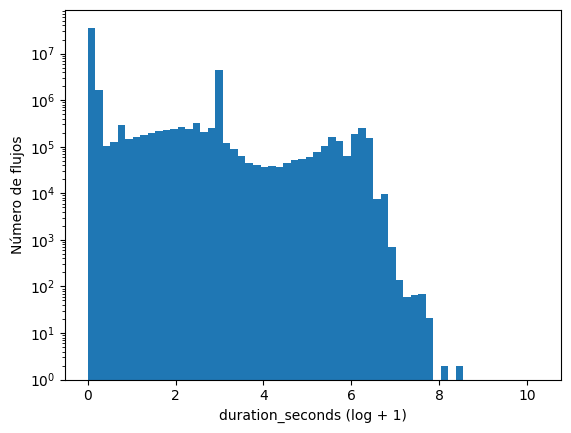
\includegraphics[width=\textwidth]{media/packet_pincer_cicddos/duration_seconds_log_x_log_y.png}
        \caption{CIC-DDoS2019}
    \end{subfigure}
    \hfill
    \begin{subfigure}[b]{0.32\textwidth}
        \centering
        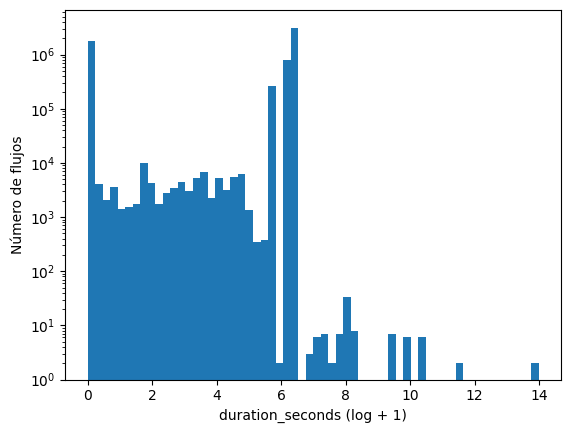
\includegraphics[width=\linewidth]{media/packet_pincer_botiot/duration_seconds_log_x_log_y.png}
        \caption{BoT-IoT}
    \end{subfigure}
    \hfill
    \begin{subfigure}[b]{0.32\textwidth}
        \centering
        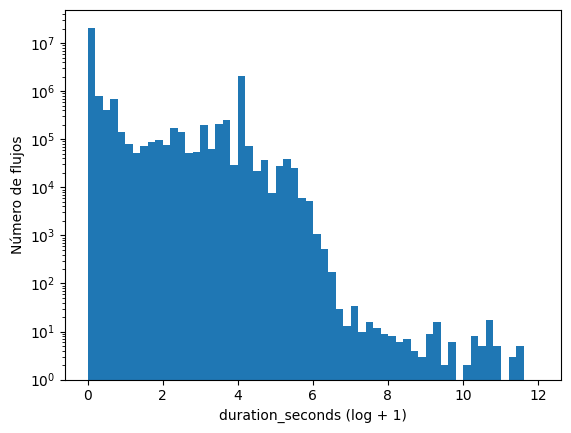
\includegraphics[width=\linewidth]{media/packet_pincer_toniot/duration_seconds_log_x_log_y.png}
        \caption{TON-IoT}
    \end{subfigure}
       \caption{Distribución de la duración de los flujos}
       \label{fig:packet_pincer_duration}
\end{figure}

\subsubsection{Recuento paquetes}

\begin{figure}[H]
    \centering
    \hfill
    \begin{subfigure}[b]{0.26\textwidth}
        \centering
        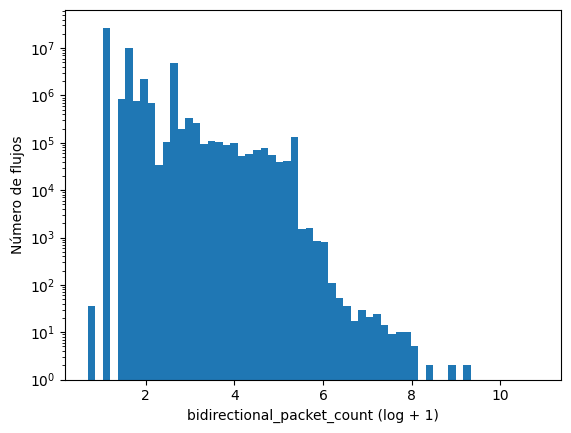
\includegraphics[width=\textwidth]{media/packet_pincer_cicddos/bidirectional_packet_count_log_x_log_y.png}
        \caption{CD (bidir.)}
        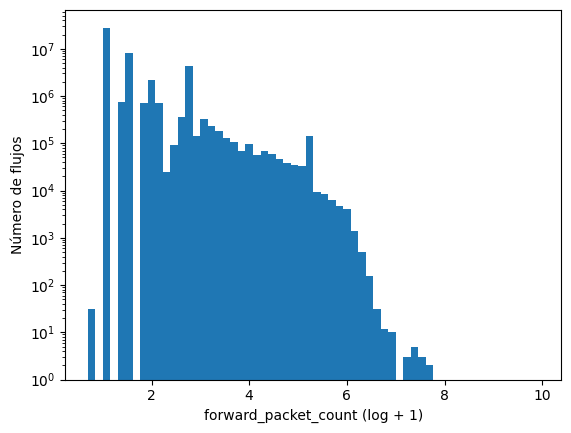
\includegraphics[width=\textwidth]{media/packet_pincer_cicddos/forward_packet_count_log_x_log_y.png}
        \caption{CD (forward)}
        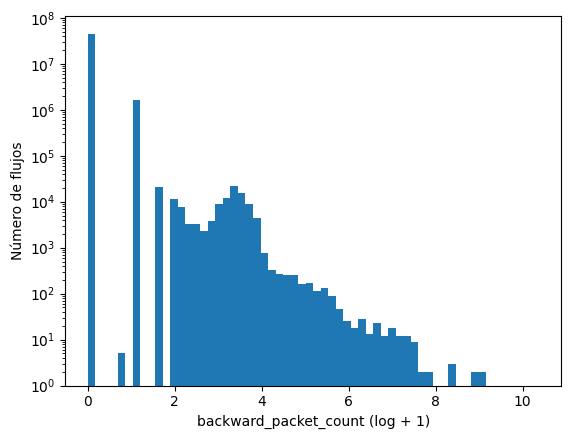
\includegraphics[width=\textwidth]{media/packet_pincer_cicddos/backward_packet_count_log_x_log_y.png}
        \caption{CD (backward)}
    \end{subfigure}
    \hfill
    \begin{subfigure}[b]{0.26\textwidth}
        \centering
        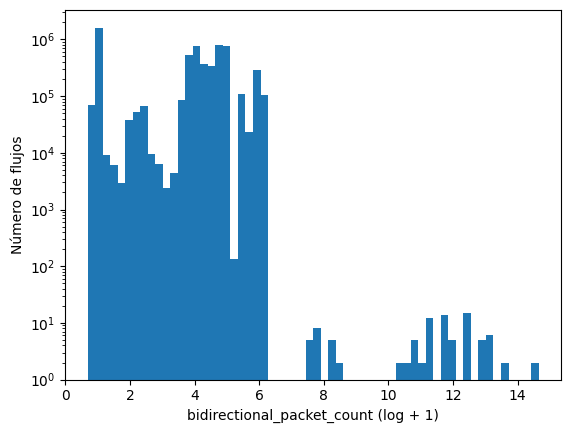
\includegraphics[width=\linewidth]{media/packet_pincer_botiot/bidirectional_packet_count_log_x_log_y.png}
        \caption{BI (bidir.)}
        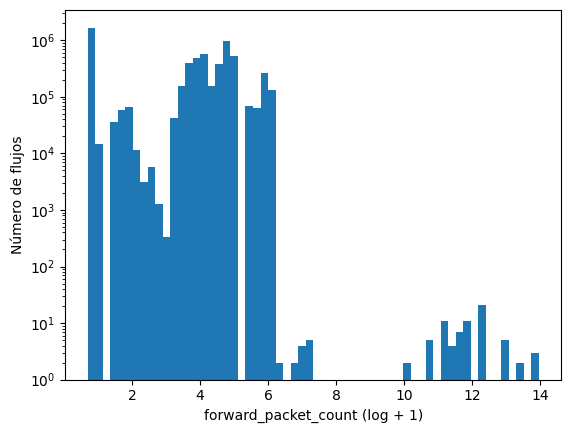
\includegraphics[width=\textwidth]{media/packet_pincer_botiot/forward_packet_count_log_x_log_y.png}
        \caption{BI (forward)}
        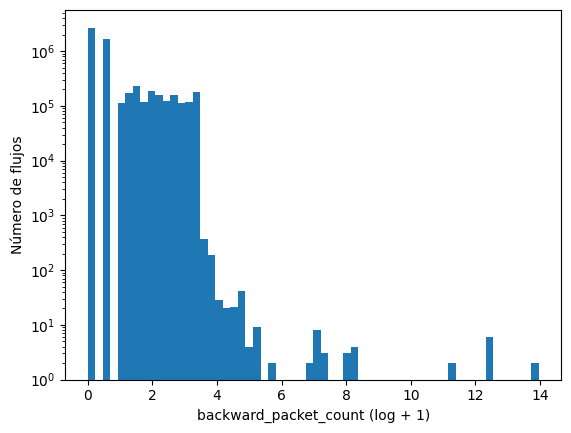
\includegraphics[width=\textwidth]{media/packet_pincer_botiot/backward_packet_count_log_x_log_y.png}
        \caption{BI (backward)}
    \end{subfigure}
    \hfill
    \begin{subfigure}[b]{0.26\textwidth}
        \centering
        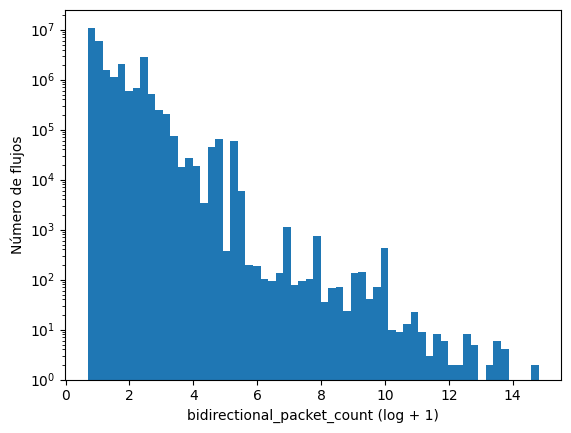
\includegraphics[width=\linewidth]{media/packet_pincer_toniot/bidirectional_packet_count_log_x_log_y.png}
        \caption{TI (bidir.)}
        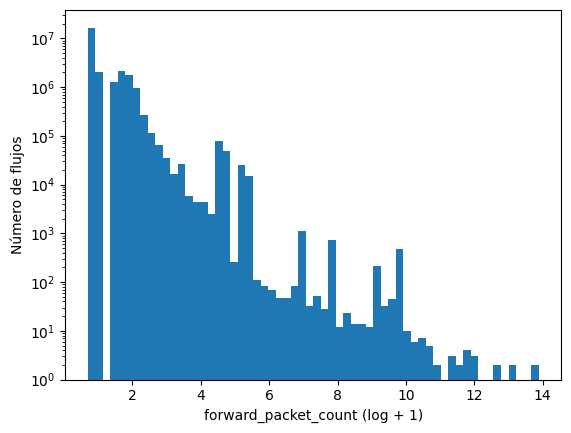
\includegraphics[width=\textwidth]{media/packet_pincer_toniot/forward_packet_count_log_x_log_y.png}
        \caption{TI (forward)}
        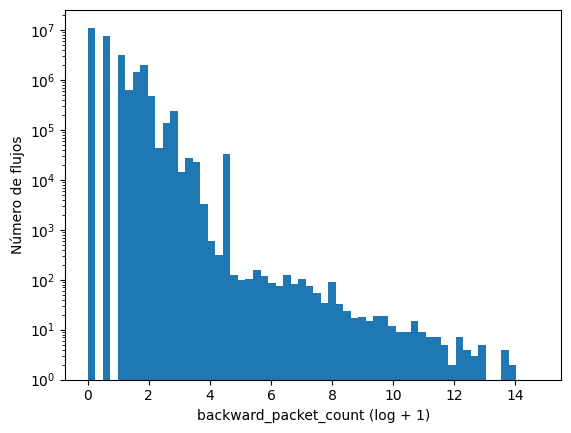
\includegraphics[width=\textwidth]{media/packet_pincer_toniot/backward_packet_count_log_x_log_y.png}
        \caption{TI (backward)}
    \end{subfigure}
    \hfill
       \caption{Distribución del número de paquetes}
       \label{fig:packet_pincer_packet_count}
\end{figure}

Podemos observar en la Figura \ref{fig:packet_pincer_packet_count} que tenemos una situación parecida al caso de la duración con el recuento de paquetes. La mayoría de los flujos tienen una cantidad de paquetes intercambiados reducida. Adicionalmente, en la mayoría hay una caída clara a partir de un punto, aunque en otros es más progresivo. Para CIC-DDoS2019 (CD en la figura) y en ToN-IoT (TI en la figura), podemos observar cierta tendencia que predice la ley de Zipf.

En este caso, para la columna del recuento de paquetes de regreso, tenemos que la cantidad de ceros es el 96.19\% (45 363 137), 44.38\% (2696542) y 43.73\% (11 211 906) en CIC-DDoS2019, BoT-Iot y TON-IoT, respectivamente.  Las otras dos no contienen ningún cero, debido a que si fuesen cero, el flujo no aparecería en los datos procesados.

\subsubsection{Cadencia paquetes}

\begin{figure}[H]
    \centering
    \hfill
    \begin{subfigure}[b]{0.26\textwidth}
        \centering
        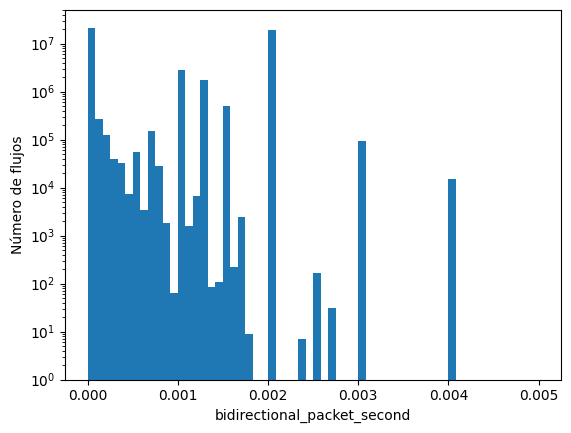
\includegraphics[width=\textwidth]{media/packet_pincer_cicddos/bidirectional_packet_second_linear_x_log_y.png}
        \caption{CD (bidir.)}
        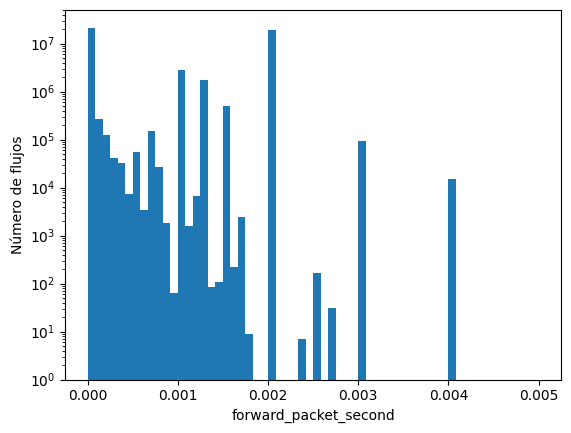
\includegraphics[width=\textwidth]{media/packet_pincer_cicddos/forward_packet_second_linear_x_log_y.png}
        \caption{CD (forward)}
        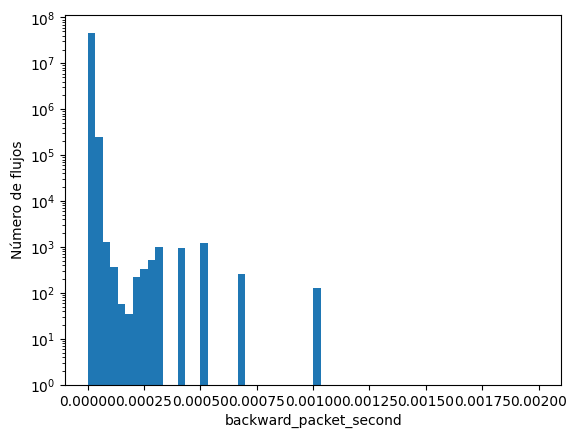
\includegraphics[width=\textwidth]{media/packet_pincer_cicddos/backward_packet_second_linear_x_log_y.png}
        \caption{CD (backward)}
    \end{subfigure}
    \hfill
    \begin{subfigure}[b]{0.26\textwidth}
        \centering
        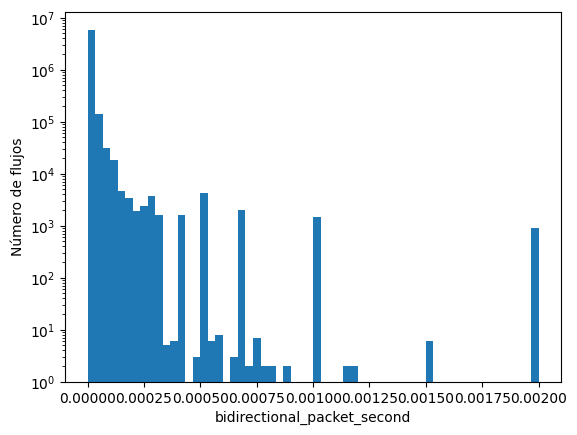
\includegraphics[width=\linewidth]{media/packet_pincer_botiot/bidirectional_packet_second_linear_x_log_y.png}
        \caption{BI (bidir.)}
        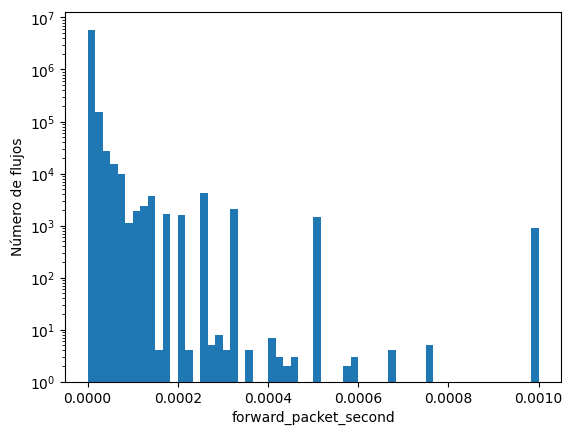
\includegraphics[width=\textwidth]{media/packet_pincer_botiot/forward_packet_second_linear_x_log_y.png}
        \caption{BI (forward)}
        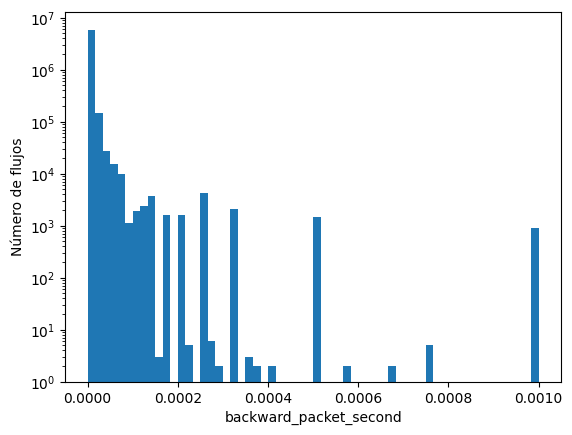
\includegraphics[width=\textwidth]{media/packet_pincer_botiot/backward_packet_second_linear_x_log_y.png}
        \caption{BI (backward)}
    \end{subfigure}
    \hfill
    \begin{subfigure}[b]{0.26\textwidth}
        \centering
        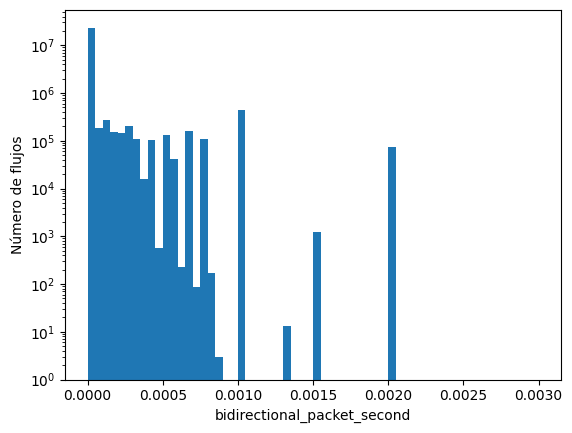
\includegraphics[width=\linewidth]{media/packet_pincer_toniot/bidirectional_packet_second_linear_x_log_y.png}
        \caption{TI (bidir.)}
        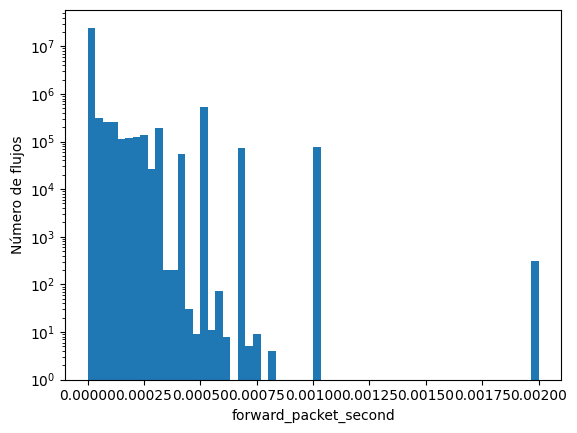
\includegraphics[width=\textwidth]{media/packet_pincer_toniot/forward_packet_second_linear_x_log_y.png}
        \caption{TI (forward)}
        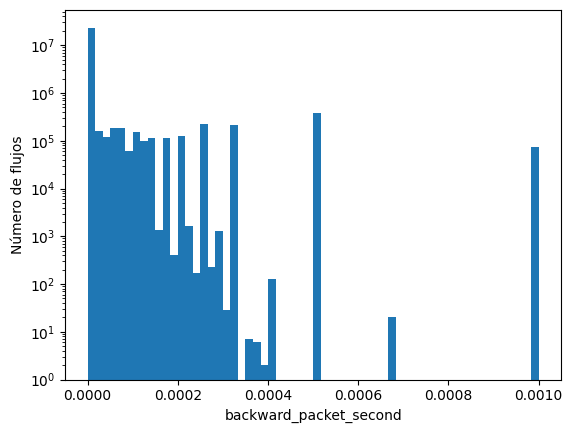
\includegraphics[width=\textwidth]{media/packet_pincer_toniot/backward_packet_second_linear_x_log_y.png}
        \caption{TI (backward)}
    \end{subfigure}
    \hfill
       \caption{Distribución de la cadencia de paquetes}
       \label{fig:packet_pincer_packet_second}
\end{figure}

La distribución de las diferentes cadencias de paquetes se puede observar en la Figura \ref{fig:packet_pincer_packet_second}. Podemos ver que la mayoría de los flujos tiene una cadencia baja, con algunos puntos con picos. En la Tabla \ref{table:packet_pincer_packet_second_zeroes} podemos ver que también hay gran cantidad de ceros en el dataset, especialmente en los IoT y en los casos de retorno. Es posible que esto haya sido debido a muchos paquetes que no hayan tenido respuesta.

\begin{table}[H]
    \centering
    \begin{tabular}{|c | c c c |}
        \hline
        \textbf{Conjunto de datos} & \textbf{Bidirectional} & \textbf{Forward} & \textbf{Backward} \\ \hline
        CIC-DDoS2019               & 8,04\%                 & 8,06\%           & 96,47\% \\
        Bot-IoT                    & 64,39\%                & 64,53\%          & 71,14\% \\
        TON-IoT                    & 53,35\%                & 54,68\%          & 55,51\% \\
        \hline
    \end{tabular}
    \caption{Protocolo de transporte utilizado por conjunto de datos}
    \label{table:packet_pincer_packet_second_zeroes}
\end{table}

\subsubsection{Número de bytes transmitidos por flujo}

\begin{figure}[H]
    \centering
    \hfill
    \begin{subfigure}[b]{0.26\textwidth}
        \centering
        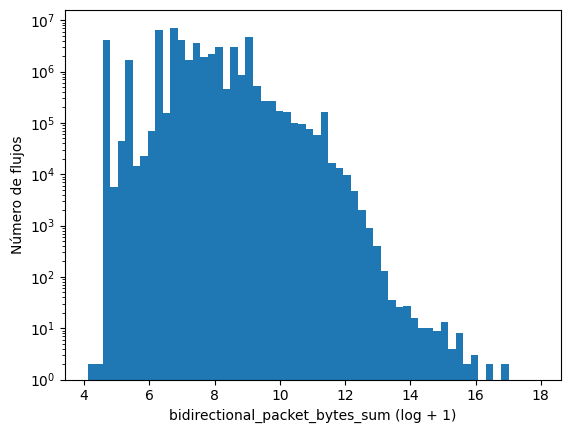
\includegraphics[width=\textwidth]{media/packet_pincer_cicddos/bidirectional_packet_bytes_sum_log_x_log_y.png}
        \caption{CD (bidir.)}
        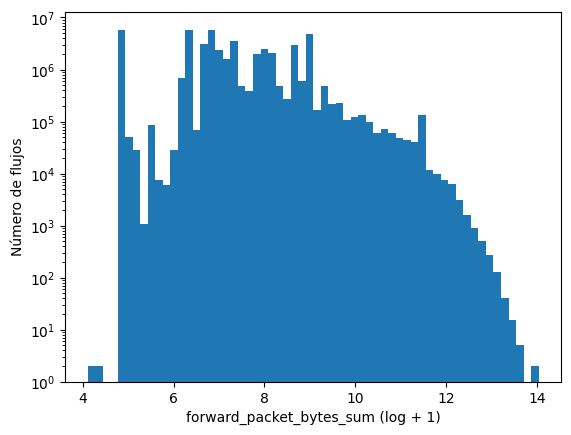
\includegraphics[width=\textwidth]{media/packet_pincer_cicddos/forward_packet_bytes_sum_log_x_log_y.png}
        \caption{CD (forward)}
        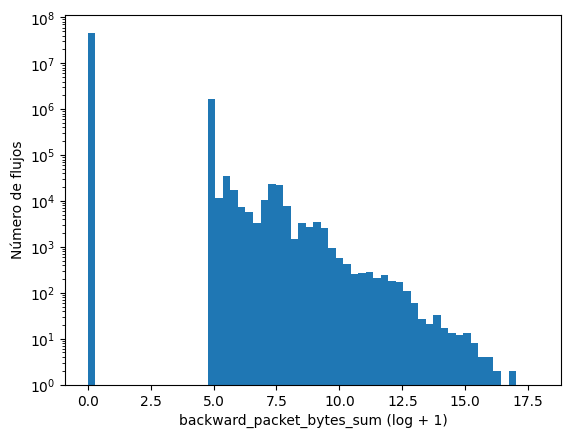
\includegraphics[width=\textwidth]{media/packet_pincer_cicddos/backward_packet_bytes_sum_log_x_log_y.png}
        \caption{CD (backward)}
    \end{subfigure}
    \hfill
    \begin{subfigure}[b]{0.26\textwidth}
        \centering
        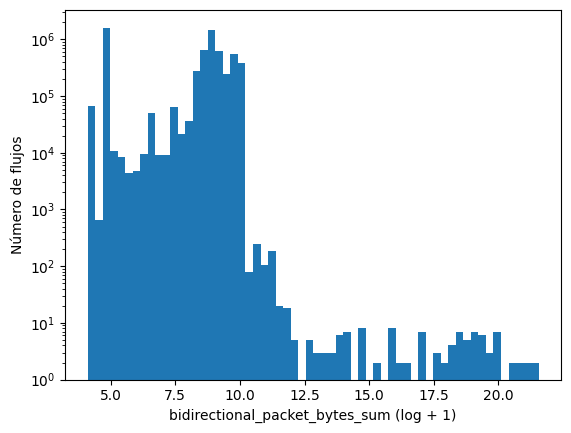
\includegraphics[width=\linewidth]{media/packet_pincer_botiot/bidirectional_packet_bytes_sum_log_x_log_y.png}
        \caption{BI (bidir.)}
        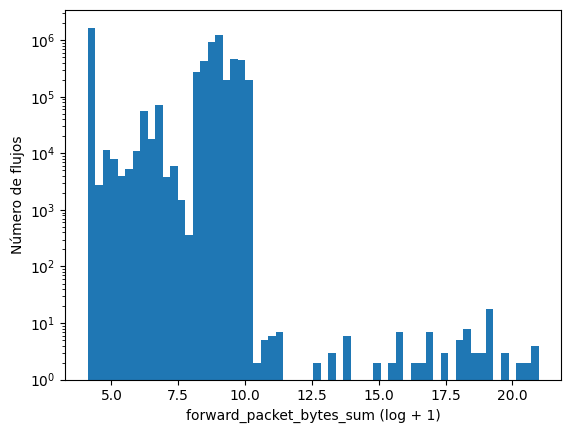
\includegraphics[width=\textwidth]{media/packet_pincer_botiot/forward_packet_bytes_sum_log_x_log_y.png}
        \caption{BI (forward)}
        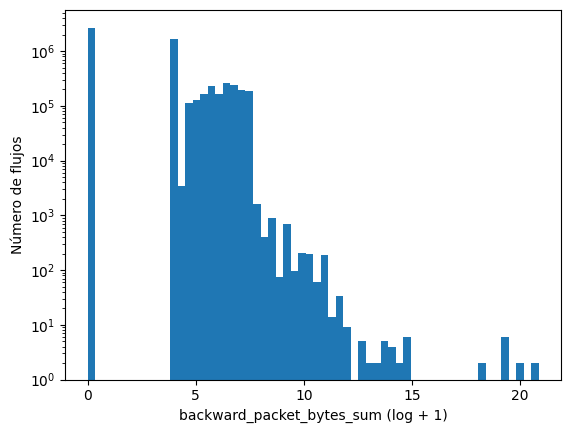
\includegraphics[width=\textwidth]{media/packet_pincer_botiot/backward_packet_bytes_sum_log_x_log_y.png}
        \caption{BI (backward)}
    \end{subfigure}
    \hfill
    \begin{subfigure}[b]{0.26\textwidth}
        \centering
        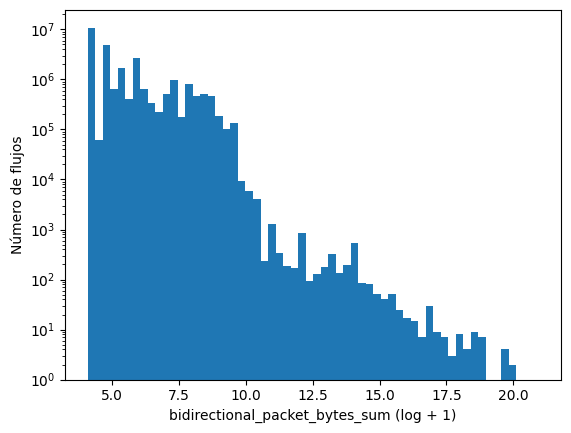
\includegraphics[width=\linewidth]{media/packet_pincer_toniot/bidirectional_packet_bytes_sum_log_x_log_y.png}
        \caption{TI (bidir.)}
        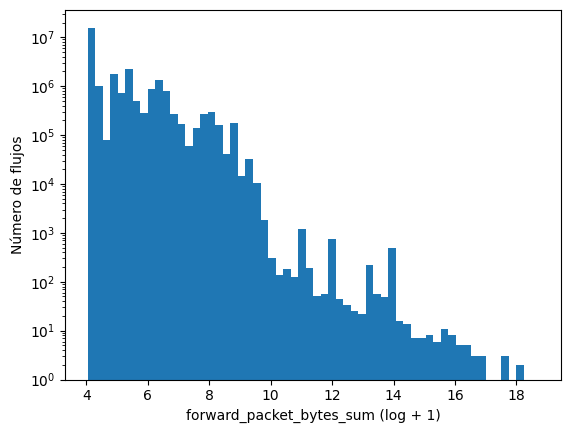
\includegraphics[width=\textwidth]{media/packet_pincer_toniot/forward_packet_bytes_sum_log_x_log_y.png}
        \caption{TI (forward)}
        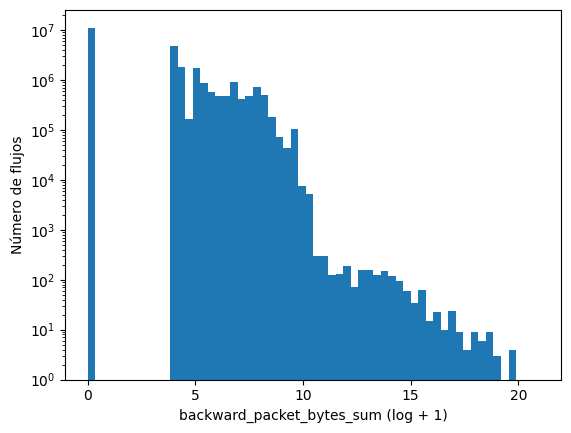
\includegraphics[width=\textwidth]{media/packet_pincer_toniot/backward_packet_bytes_sum_log_x_log_y.png}
        \caption{TI (backward)}
    \end{subfigure}
    \hfill
       \caption{Distribución de la suma de bytes transmitidas por flujo}
       \label{fig:packet_pincer_packet_bytes_sum}
\end{figure}

La distribución de las sumas totales de los bytes transmitidos por cada flujo está representada en la Figura \ref{fig:packet_pincer_packet_bytes_sum}. Podemos ver que en algunos casos la distribución parece marcada por la ley the Zipf, pero otro se asemeja más a una distribución normal al expresarlo en una gráfica log-log. Adicionalmente, en otros tenemos una caída notable a partir de cierto punto. Aparte de las peticiones que no reciben respuesta, no hay registros con ceros.

\subsubsection{Número de bytes máximos por flujo}

Si observamos las distribuciones de los bytes máximos en paquetes por flujo representadas en la Figura \ref{fig:packet_pincer_packet_bytes_max}, podemos ver que en general son similares. Sin embargo, las respuestas (backward) en CIC-DDos2019 (CD en la figura), la 'cola' de la distribución parece haber sido cortada. Adicionalmente, en los otros dos conjuntos de datos los picos son menos pronunciados en este caso.

\begin{figure}[H]
    \centering
    \hfill
    \begin{subfigure}[b]{0.26\textwidth}
        \centering
        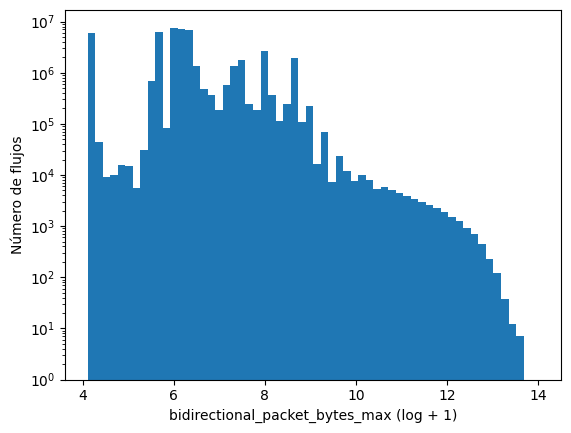
\includegraphics[width=\textwidth]{media/packet_pincer_cicddos/bidirectional_packet_bytes_max_log_x_log_y.png}
        \caption{CD (bidir.)}
        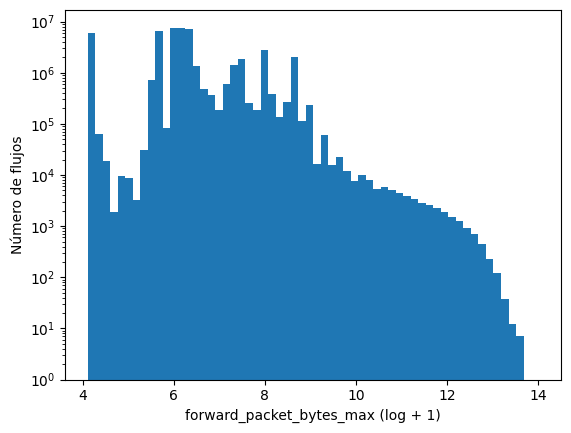
\includegraphics[width=\textwidth]{media/packet_pincer_cicddos/forward_packet_bytes_max_log_x_log_y.png}
        \caption{CD (forward)}
        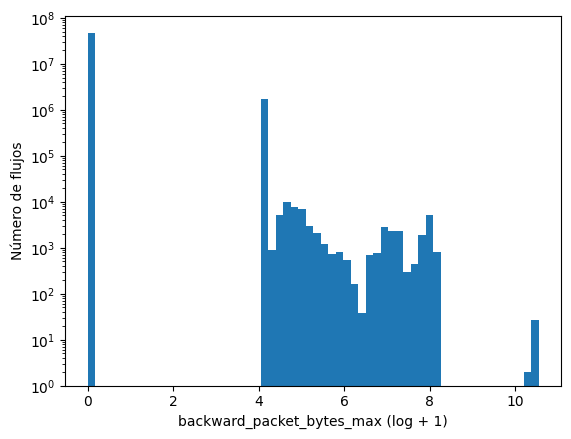
\includegraphics[width=\textwidth]{media/packet_pincer_cicddos/backward_packet_bytes_max_log_x_log_y.png}
        \caption{CD (backward)}
    \end{subfigure}
    \hfill
    \begin{subfigure}[b]{0.26\textwidth}
        \centering
        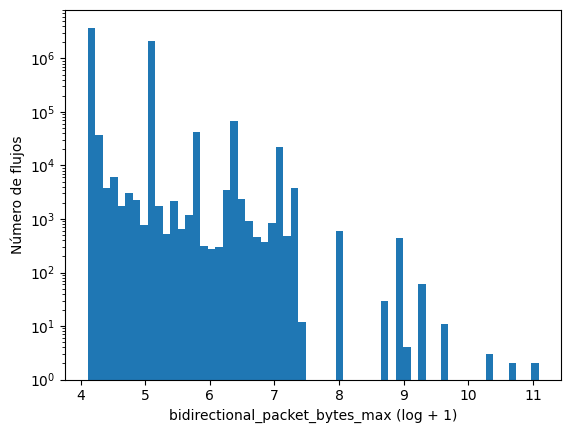
\includegraphics[width=\linewidth]{media/packet_pincer_botiot/bidirectional_packet_bytes_max_log_x_log_y.png}
        \caption{BI (bidir.)}
        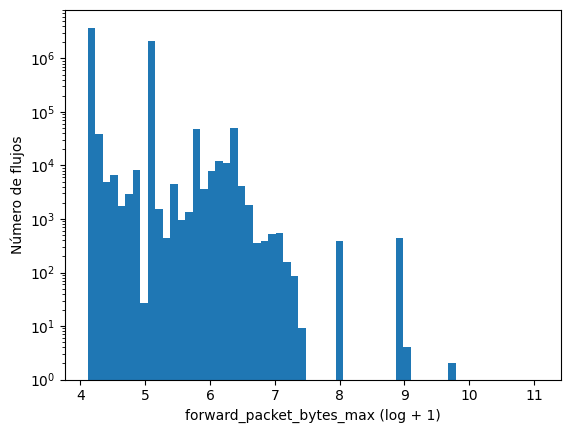
\includegraphics[width=\textwidth]{media/packet_pincer_botiot/forward_packet_bytes_max_log_x_log_y.png}
        \caption{BI (forward)}
        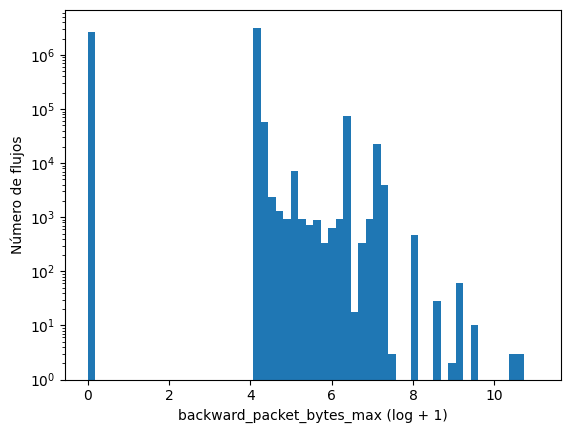
\includegraphics[width=\textwidth]{media/packet_pincer_botiot/backward_packet_bytes_max_log_x_log_y.png}
        \caption{BI (backward)}
    \end{subfigure}
    \hfill
    \begin{subfigure}[b]{0.26\textwidth}
        \centering
        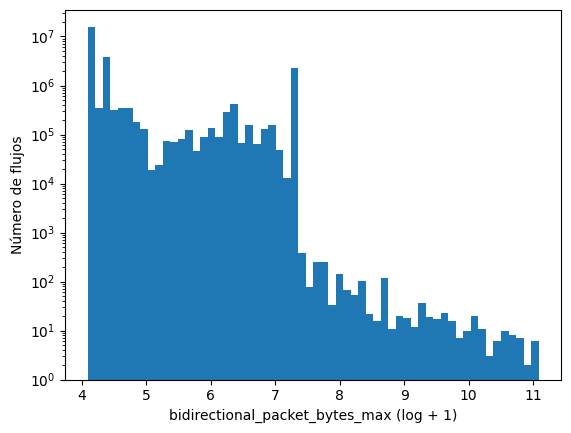
\includegraphics[width=\linewidth]{media/packet_pincer_toniot/bidirectional_packet_bytes_max_log_x_log_y.png}
        \caption{TI (bidir.)}
        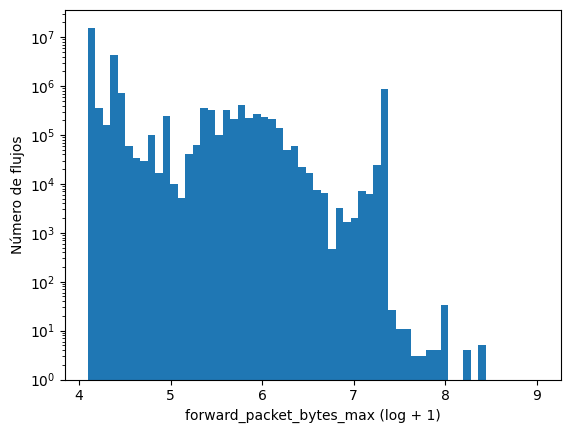
\includegraphics[width=\textwidth]{media/packet_pincer_toniot/forward_packet_bytes_max_log_x_log_y.png}
        \caption{TI (forward)}
        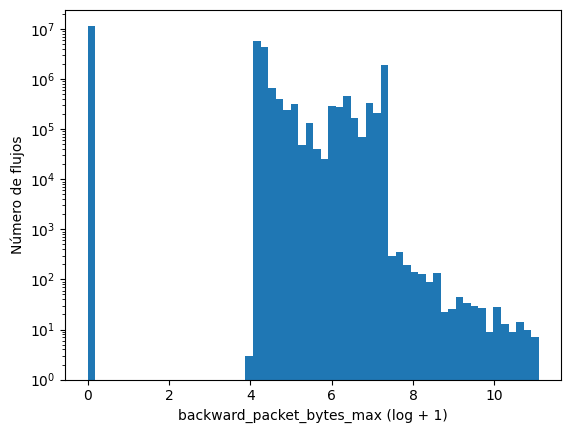
\includegraphics[width=\textwidth]{media/packet_pincer_toniot/backward_packet_bytes_max_log_x_log_y.png}
        \caption{TI (backward)}
    \end{subfigure}
    \hfill
       \caption{Distribución de los máximos bytes transmitidos en un paquete por flujo}
       \label{fig:packet_pincer_packet_bytes_max}
\end{figure}

\subsubsection{Número de bytes mínimos por flujo}

Para el caso de bytes mínimos en paquetes, podemos ver que en la Figura \ref{fig:packet_pincer_packet_bytes_min} nos encontramos con un caso similar al caso de los máximos. Sin embargo, para el caso de CIC-DDoS, el corte es en una magnitud menor y en los otros parece haber más huecos y concentraciones en ciertos puntos de la distribución.

\begin{figure}[H]
    \centering
    \hfill
    \begin{subfigure}[b]{0.26\textwidth}
        \centering
        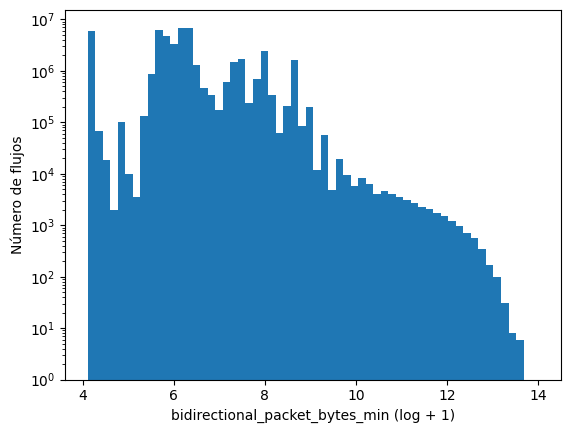
\includegraphics[width=\textwidth]{media/packet_pincer_cicddos/bidirectional_packet_bytes_min_log_x_log_y.png}
        \caption{CD (bidir.)}
        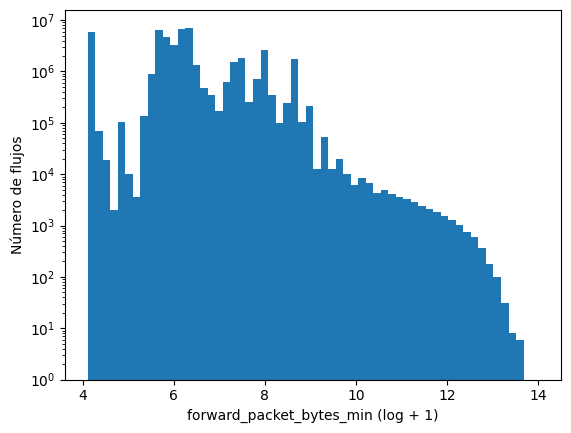
\includegraphics[width=\textwidth]{media/packet_pincer_cicddos/forward_packet_bytes_min_log_x_log_y.png}
        \caption{CD (forward)}
        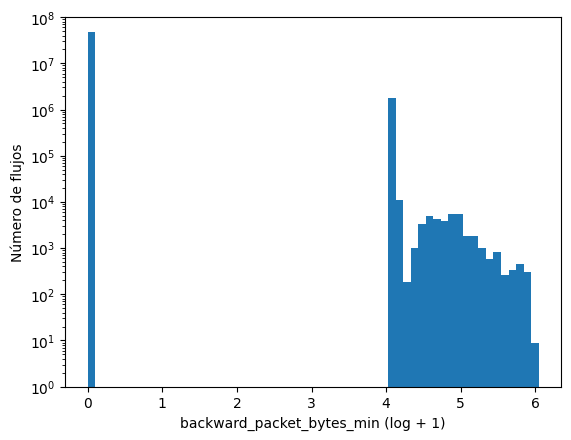
\includegraphics[width=\textwidth]{media/packet_pincer_cicddos/backward_packet_bytes_min_log_x_log_y.png}
        \caption{CD (backward)}
    \end{subfigure}
    \hfill
    \begin{subfigure}[b]{0.26\textwidth}
        \centering
        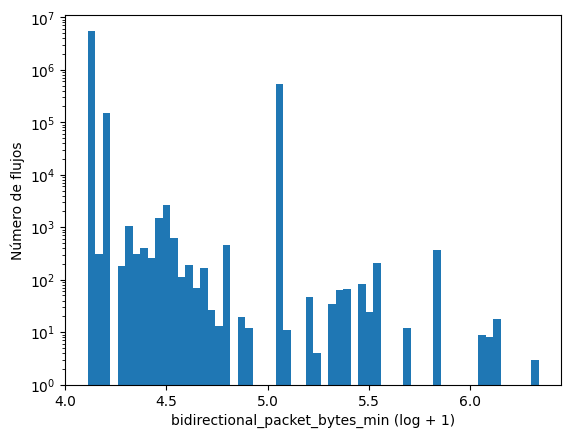
\includegraphics[width=\linewidth]{media/packet_pincer_botiot/bidirectional_packet_bytes_min_log_x_log_y.png}
        \caption{BI (bidir.)}
        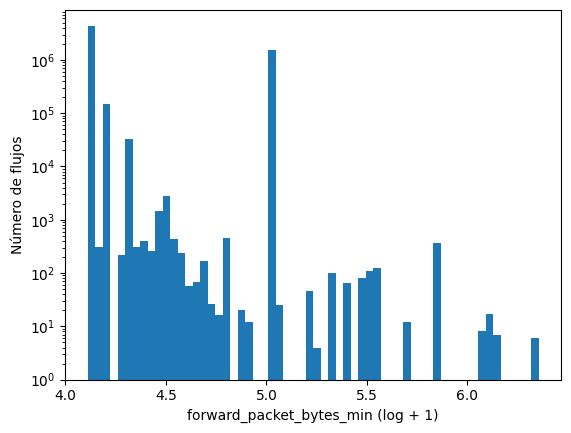
\includegraphics[width=\textwidth]{media/packet_pincer_botiot/forward_packet_bytes_min_log_x_log_y.png}
        \caption{BI (forward)}
        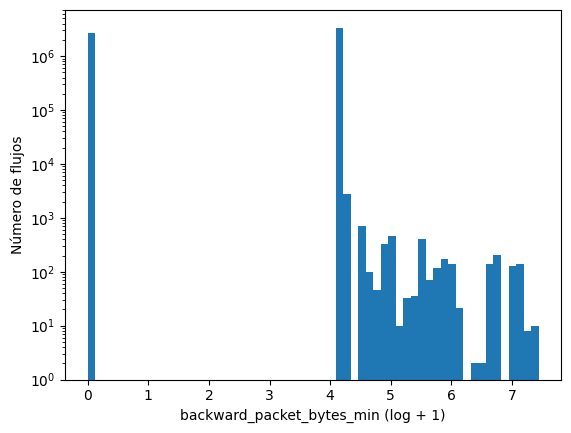
\includegraphics[width=\textwidth]{media/packet_pincer_botiot/backward_packet_bytes_min_log_x_log_y.png}
        \caption{BI (backward)}
    \end{subfigure}
    \hfill
    \begin{subfigure}[b]{0.26\textwidth}
        \centering
        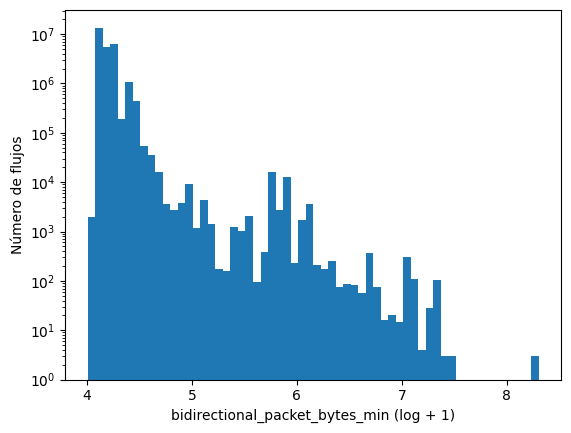
\includegraphics[width=\linewidth]{media/packet_pincer_toniot/bidirectional_packet_bytes_min_log_x_log_y.png}
        \caption{TI (bidir.)}
        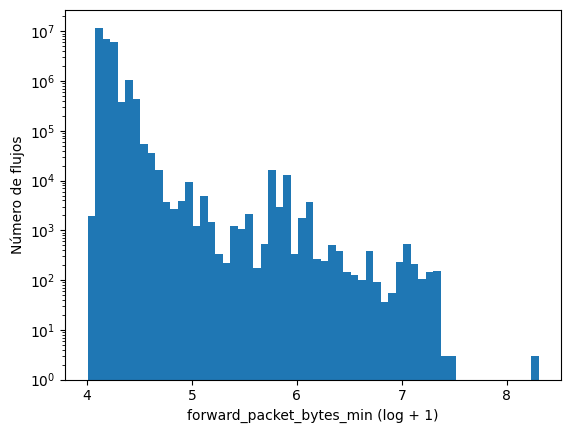
\includegraphics[width=\textwidth]{media/packet_pincer_toniot/forward_packet_bytes_min_log_x_log_y.png}
        \caption{TI (forward)}
        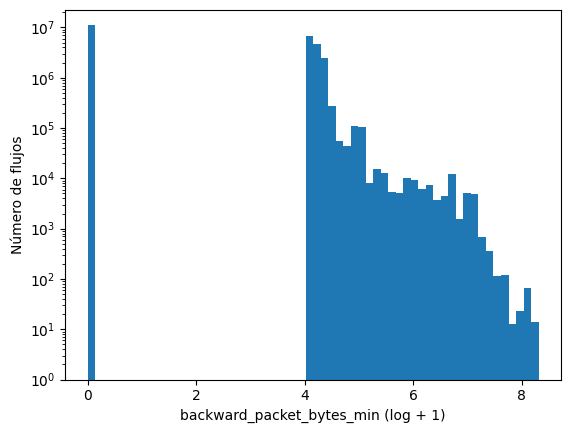
\includegraphics[width=\textwidth]{media/packet_pincer_toniot/backward_packet_bytes_min_log_x_log_y.png}
        \caption{TI (backward)}
    \end{subfigure}
    \hfill
       \caption{Distribución de los máximos bytes transmitidos en un paquete por flujo}
       \label{fig:packet_pincer_packet_bytes_min}
\end{figure}

\subsubsection{Número de bytes medio por flujo}

Las distribuciones de los bytes medios de la Figura \ref{fig:packet_pincer_packet_bytes_mean} se asemejan a las de los recuentos de los bytes totales, pero suavizadas. Podemos ver que, en el caso bidireccional de TON-IoT (TI en la figura), la gráfica se mantiene en número de flujos alto durante un mayor rango de medias antes de caer.

\begin{figure}[H]
    \centering
    \hfill
    \begin{subfigure}[b]{0.26\textwidth}
        \centering
        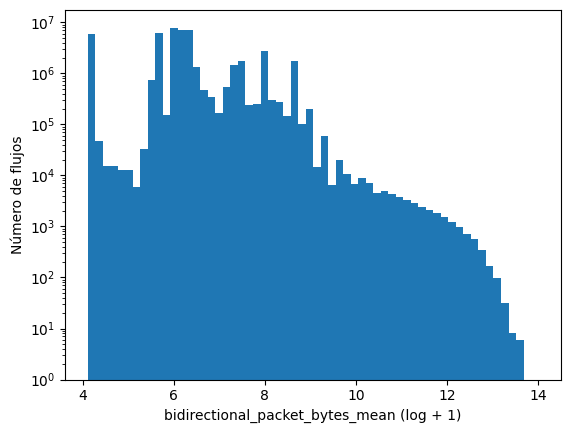
\includegraphics[width=\textwidth]{media/packet_pincer_cicddos/bidirectional_packet_bytes_mean_log_x_log_y.png}
        \caption{CD (bidir.)}
        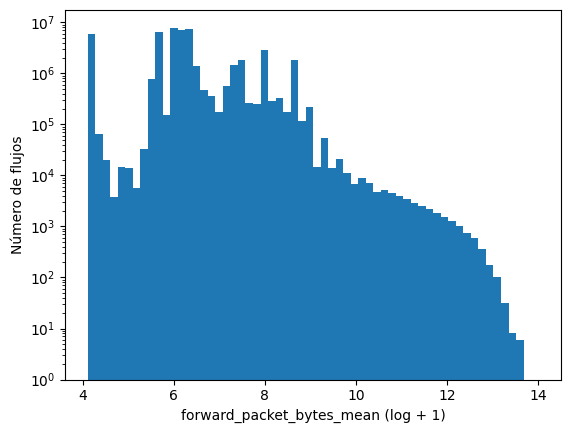
\includegraphics[width=\textwidth]{media/packet_pincer_cicddos/forward_packet_bytes_mean_log_x_log_y.png}
        \caption{CD (forward)}
        \includegraphics[width=\textwidth]{media/packet_pincer_cicddos/backward_packet_bytes_mean_log_x_log_y.png}
        \caption{CD (backward)}
    \end{subfigure}
    \hfill
    \begin{subfigure}[b]{0.26\textwidth}
        \centering
        \includegraphics[width=\linewidth]{media/packet_pincer_botiot/bidirectional_packet_bytes_mean_log_x_log_y.png}
        \caption{BI (bidir.)}
        \includegraphics[width=\textwidth]{media/packet_pincer_botiot/forward_packet_bytes_mean_log_x_log_y.png}
        \caption{BI (forward)}
        \includegraphics[width=\textwidth]{media/packet_pincer_botiot/backward_packet_bytes_mean_log_x_log_y.png}
        \caption{BI (backward)}
    \end{subfigure}
    \hfill
    \begin{subfigure}[b]{0.26\textwidth}
        \centering
        \includegraphics[width=\linewidth]{media/packet_pincer_toniot/bidirectional_packet_bytes_mean_log_x_log_y.png}
        \caption{TI (bidir.)}
        \includegraphics[width=\textwidth]{media/packet_pincer_toniot/forward_packet_bytes_mean_log_x_log_y.png}
        \caption{TI (forward)}
        \includegraphics[width=\textwidth]{media/packet_pincer_toniot/backward_packet_bytes_mean_log_x_log_y.png}
        \caption{TI (backward)}
    \end{subfigure}
    \hfill
       \caption{Distribución de los bytes medios transmitidos en un paquete por flujo}
       \label{fig:packet_pincer_packet_bytes_mean}
\end{figure}

\subsubsection{Desviación estándar del numero de bytes por flujo}

Las distribuciones de las diferentes desviaciones estándar son variadas. Tenemos en muchos casos donde la desviación es 0, la cual puede ser causada por flujos con paquetes muy iguales o los casos donde no se transmite nada, ya que se asigna 0 en ese caso. De todas formas, para todos los casos, donde no son 0, hay una variedad de distribuciones. En el caso de CIC-DDoS2019, se asemeja a sus distribuciones anteriores en el caso bidireccional y hacia el receptor inicial. Hacia el transmisor inicial está invertida, teniendo mucha variabilidad en los diferentes tamaños de las comunicaciones. La gran diferencia de variabilidad es quizá debido a los efectos del control de congestión de las transmisiones. Dependiendo del estado de la red, los diferentes dispositivos transmitirán de una forma más constante y predecible y en otras se tendrán que ir adaptando a tiempo real al nivel de congestión.

\begin{figure}[H]
    \centering
    \hfill
    \begin{subfigure}[b]{0.26\textwidth}
        \centering
        \includegraphics[width=\textwidth]{media/packet_pincer_cicddos/bidirectional_packet_bytes_std_log_x_log_y.png}
        \caption{CD (bidir.)}
        \includegraphics[width=\textwidth]{media/packet_pincer_cicddos/forward_packet_bytes_std_log_x_log_y.png}
        \caption{CD (forward)}
        \includegraphics[width=\textwidth]{media/packet_pincer_cicddos/backward_packet_bytes_std_log_x_log_y.png}
        \caption{CD (backward)}
    \end{subfigure}
    \hfill
    \begin{subfigure}[b]{0.26\textwidth}
        \centering
        \includegraphics[width=\linewidth]{media/packet_pincer_botiot/bidirectional_packet_bytes_std_log_x_log_y.png}
        \caption{BI (bidir.)}
        \includegraphics[width=\textwidth]{media/packet_pincer_botiot/forward_packet_bytes_std_log_x_log_y.png}
        \caption{BI (forward)}
        \includegraphics[width=\textwidth]{media/packet_pincer_botiot/backward_packet_bytes_std_log_x_log_y.png}
        \caption{BI (backward)}
    \end{subfigure}
    \hfill
    \begin{subfigure}[b]{0.26\textwidth}
        \centering
        \includegraphics[width=\linewidth]{media/packet_pincer_toniot/bidirectional_packet_bytes_std_log_x_log_y.png}
        \caption{TI (bidir.)}
        \includegraphics[width=\textwidth]{media/packet_pincer_toniot/forward_packet_bytes_std_log_x_log_y.png}
        \caption{TI (forward)}
        \includegraphics[width=\textwidth]{media/packet_pincer_toniot/backward_packet_bytes_std_log_x_log_y.png}
        \caption{TI (backward)}
    \end{subfigure}
    \hfill
       \caption{Desviación estándard del número de bytes transmitidos en un paquete por flujo}
       \label{fig:packet_pincer_packet_bytes_std}
\end{figure}

\subsubsection{Balance entre subida y bajada}

El balance o la razón entre la subida y bajada consiste en dividir la cantidad de bytes enviados por el receptor inicial entre los enviados por el iniciador de la comunicación. De esta manera, se puede inferir si la comunicación es principalmente de bajada (un valor inferior a 1), de subida (un valor superior a 1) o hay una comunicación a iguales. En el primer caso, se puede dar al visitar la web o descargar archivos. El segundo en casos donde se suban datos, como subir fotos a un servicio Cloud. Finalmente, el tercero podría consistir en, por ejemplo, en una llamada de voz o videoconferencia. 

Podemos en la figura \ref{fig:packet_pincer_down_up_bytes_ratio} que la gran mayoría de comunicaciones se concentran en la parte baja del gráfico, indicando que suelen ser o de bajada o la cantidad de datos enviados no suele ser muy grande. Sin embargo, hay una cantidad relevante de flujos en la que el emisor de la comunicación envía muchos más datos de los que recibe. Esto puede estar relacionado con posibles ataques, donde las comunicaciones normales tienen un ratio más bajo.

\begin{figure}[H]
    \centering
    \begin{subfigure}[b]{0.32\textwidth}
        \centering
        \includegraphics[width=\textwidth]{media/packet_pincer_cicddos/down_up_bytes_ratio_log_x_log_y.png}
        \caption{CIC-DDoS2019}
    \end{subfigure}
    \hfill
    \begin{subfigure}[b]{0.32\textwidth}
        \centering
        \includegraphics[width=\linewidth]{media/packet_pincer_botiot/down_up_bytes_ratio_log_x_log_y.png}
        \caption{BoT-IoT}
    \end{subfigure}
    \hfill
    \begin{subfigure}[b]{0.32\textwidth}
        \centering
        \includegraphics[width=\linewidth]{media/packet_pincer_toniot/down_up_bytes_ratio_log_x_log_y.png}
        \caption{TON-IoT}
    \end{subfigure}
       \caption{Distribución del balance de los flujos}
       \label{fig:packet_pincer_down_up_bytes_ratio}
\end{figure}

\subsubsection{Cadencia datos}

\begin{figure}[H]
    \centering
    \hfill
    \begin{subfigure}[b]{0.26\textwidth}
        \centering
        \includegraphics[width=\textwidth]{media/packet_pincer_cicddos/bidirectional_bytes_s_log_x_log_y.png}
        \caption{CD (bidir.)}
        \includegraphics[width=\textwidth]{media/packet_pincer_cicddos/forward_bytes_s_log_x_log_y.png}
        \caption{CD (forward)}
        \includegraphics[width=\textwidth]{media/packet_pincer_cicddos/backward_bytes_s_log_x_log_y.png}
        \caption{CD (backward)}
    \end{subfigure}
    \hfill
    \begin{subfigure}[b]{0.26\textwidth}
        \centering
        \includegraphics[width=\linewidth]{media/packet_pincer_botiot/bidirectional_bytes_s_log_x_log_y.png}
        \caption{BI (bidir.)}
        \includegraphics[width=\textwidth]{media/packet_pincer_botiot/forward_bytes_s_log_x_log_y.png}
        \caption{BI (forward)}
        \includegraphics[width=\textwidth]{media/packet_pincer_botiot/backward_bytes_s_log_x_log_y.png}
        \caption{BI (backward)}
    \end{subfigure}
    \hfill
    \begin{subfigure}[b]{0.26\textwidth}
        \centering
        \includegraphics[width=\linewidth]{media/packet_pincer_toniot/bidirectional_bytes_s_log_x_log_y.png}
        \caption{TI (bidir.)}
        \includegraphics[width=\textwidth]{media/packet_pincer_toniot/forward_bytes_s_log_x_log_y.png}
        \caption{TI (forward)}
        \includegraphics[width=\textwidth]{media/packet_pincer_toniot/backward_bytes_s_log_x_log_y.png}
        \caption{TI (backward)}
    \end{subfigure}
    \hfill
       \caption{Cadencia de bytes medios por flujo}
       \label{fig:packet_pincer_bytes_s}
\end{figure}

En la Figura \ref{fig:packet_pincer_bytes_s} podemos ver la distribución de las diferentes cadencias medias de bytes transmitidos por flujos. Podemos observar que hay mayor variedad en el caso de CIC-DDoS2019, mientras que en las otras los valores son más bajos y se encuentran más concentrados. Estos valores pueden aportar información sobre transmisiones en las que haya habido mayor o menor actividad.

\subsubsection{Tiempo de llegada máxima}

\begin{figure}[H]
    \centering
    \hfill
    \begin{subfigure}[b]{0.26\textwidth}
        \centering
        \includegraphics[width=\textwidth]{media/packet_pincer_cicddos/bidirectional_inter_arrival_time_max_log_x_log_y.png}
        \caption{CD (bidir.)}
        \includegraphics[width=\textwidth]{media/packet_pincer_cicddos/forward_inter_arrival_time_max_log_x_log_y.png}
        \caption{CD (forward)}
        \includegraphics[width=\textwidth]{media/packet_pincer_cicddos/backward_inter_arrival_time_max_log_x_log_y.png}
        \caption{CD (backward)}
    \end{subfigure}
    \hfill
    \begin{subfigure}[b]{0.26\textwidth}
        \centering
        \includegraphics[width=\linewidth]{media/packet_pincer_botiot/bidirectional_inter_arrival_time_max_log_x_log_y.png}
        \caption{BI (bidir.)}
        \includegraphics[width=\textwidth]{media/packet_pincer_botiot/forward_inter_arrival_time_max_log_x_log_y.png}
        \caption{BI (forward)}
        \includegraphics[width=\textwidth]{media/packet_pincer_botiot/backward_inter_arrival_time_max_log_x_log_y.png}
        \caption{BI (backward)}
    \end{subfigure}
    \hfill
    \begin{subfigure}[b]{0.26\textwidth}
        \centering
        \includegraphics[width=\linewidth]{media/packet_pincer_toniot/bidirectional_inter_arrival_time_max_log_x_log_y.png}
        \caption{TI (bidir.)}
        \includegraphics[width=\textwidth]{media/packet_pincer_toniot/forward_inter_arrival_time_max_log_x_log_y.png}
        \caption{TI (forward)}
        \includegraphics[width=\textwidth]{media/packet_pincer_toniot/backward_inter_arrival_time_max_log_x_log_y.png}
        \caption{TI (backward)}
    \end{subfigure}
    \hfill
       \caption{Distribución del número de paquetes}
       \label{fig:packet_pincer_inter_arrival_time_max}
\end{figure}

La distribución de los tiempos de llegada máxima entre paquetes la podemos observar en la Figura \ref{fig:packet_pincer_inter_arrival_time_max}. Podemos ver que en los casos de CIC-DDoS2019 y TON-IOT, aparte de los ceros, se encuentra relativamente repartido. En cambio, en BoT-IoT hay una acumulación clara en cierto punto de la gráfica.

\subsubsection{Tiempo de llegada mínima}

por hacer
%"bidirectional_inter_arrival_time_min","forward_inter_arrival_time_min","backward_inter_arrival_time_min",

\subsubsection{Tiempo de llegada media}

por hacer
%"bidirectional_inter_arrival_time_mean","forward_inter_arrival_time_mean","backward_inter_arrival_time_mean",

\subsubsection{Variación de los tiempos de llegada}

por hacer
%"bidirectional_inter_arrival_time_std","forward_inter_arrival_time_std","backward_inter_arrival_time_std",

\subsubsection{Flags cabecera TCP}

por hacer
%"bidirectional_tcp_cwr_flags_count",
%"bidirectional_tcp_ece_flags_count",
%"bidirectional_tcp_urg_flags_count",
%"bidirectional_tcp_ack_flags_count",
%"bidirectional_tcp_psh_flags_count",
%"bidirectional_tcp_rst_flags_count",
%"bidirectional_tcp_syn_flags_count",
%"bidirectional_tcp_fin_flags_count",

%forward_tcp_psh_flags_count,backward_tcp_psh_flags_count
%"forward_tcp_urg_flags_count","backward_tcp_urg_flags_count",

\subsubsection{Suma total de bytes en las cabeceras de transporte}

por hacer
%"forward_transport_header_bytes_sum",backward_transport_header_bytes_sum

\subsubsection{Media de bytes enviados sobre la capa de transporte en un paquete}

por hacer
%"forward_transport_payload_bytes_mean",backward_transport_payload_bytes_mean

\subsubsection{Bytes mínimos enviados sobre la capa de transporte}

por hacer
%"forward_transport_payload_bytes_min",

\subsubsection{Numero de paquetes enviados con datos en la capa de transporte}

por hacer
%"forward_transport_packets_with_payload_count",

\subsubsection{Ventana TCP inicial}

por hacer
%"forward_tcp_initial_window_bytes","backward_tcp_initial_window_bytes",

\subsubsection{Tiempos de actividad mínimos}

por hacer
%"idle_seconds_min",active_seconds_min

\subsubsection{Tiempos de actividad máximos}

por hacer
%""idle_seconds_max",active_seconds_max

\subsubsection{Tiempos de actividad medios}

por hacer
%""idle_seconds_mean",active_seconds_mean

\subsubsection{Variación de tiempos de actividad}

por hacer
%""idle_seconds_std"active_seconds_std

\subsubsection{Media de paquetes por grupo activo}

por hacer
%"active_group_forward_packet_average","active_group_backward_packet_average",

\subsubsection{Media de bytes por grupo activo}

por hacer
%"active_group_forward_byte_average","active_group_backward_byte_average",

\subsubsection{Cadencia de bytes por grupo activo}

por hacer
%"active_group_forward_byte_second_average","active_group_backward_byte_second_average"

\subsection{Definición y evaluación de la tarea a realizar}

por hacer

\subsection{Preprocessamiento}

\subsubsection{Combinación etiquetas}
por hacer

\subsubsection{Omisión de características inicial}
por hacer

\subsubsection{Escalado y normalización}
por hacer

\subsubsection{Selección de características?}
por hacer

\subsubsection{Reducción dimensionalidad?}
por hacer

\subsection{Entrenamiento de modelos}

por hacer

\subsection{Comparación de resultados}

por hacer

